% Template for PLoS
% Version 3.5 March 2018
%
% % % % % % % % % % % % % % % % % % % % % %
%
% -- IMPORTANT NOTE
%
% This template contains comments intended
% to minimize problems and delays during our production
% process. Please follow the template instructions
% whenever possible.
%
% % % % % % % % % % % % % % % % % % % % % % %
%
% Once your paper is accepted for publication,
% PLEASE REMOVE ALL TRACKED CHANGES in this file
% and leave only the final text of your manuscript.
% PLOS recommends the use of latexdiff to track changes during review, as this will help to maintain a clean tex file.
% Visit https://www.ctan.org/pkg/latexdiff?lang=en for info or contact us at latex@plos.org.
%
%
% There are no restrictions on package use within the LaTeX files except that
% no packages listed in the template may be deleted.
%
% Please do not include colors or graphics in the text.
%
% The manuscript LaTeX source should be contained within a single file (do not use \input, \externaldocument, or similar commands).
%
% % % % % % % % % % % % % % % % % % % % % % %
%
% -- FIGURES AND TABLES
%
% Please include tables/figure captions directly after the paragraph where they are first cited in the text.
%
% DO NOT INCLUDE GRAPHICS IN YOUR MANUSCRIPT
% - Figures should be uploaded separately from your manuscript file.
% - Figures generated using LaTeX should be extracted and removed from the PDF before submission.
% - Figures containing multiple panels/subfigures must be combined into one image file before submission.
% For figure citations, please use "Fig" instead of "Figure".
% See http://journals.plos.org/plosone/s/figures for PLOS figure guidelines.
%
% Tables should be cell-based and may not contain:
% - spacing/line breaks within cells to alter layout or alignment
% - do not nest tabular environments (no tabular environments within tabular environments)
% - no graphics or colored text (cell background color/shading OK)
% See http://journals.plos.org/plosone/s/tables for table guidelines.
%
% For tables that exceed the width of the text column, use the adjustwidth environment as illustrated in the example table in text below.
%
% % % % % % % % % % % % % % % % % % % % % % % %
%
% -- EQUATIONS, MATH SYMBOLS, SUBSCRIPTS, AND SUPERSCRIPTS
%
% IMPORTANT
% Below are a few tips to help format your equations and other special characters according to our specifications. For more tips to help reduce the possibility of formatting errors during conversion, please see our LaTeX guidelines at http://journals.plos.org/plosone/s/latex
%
% For inline equations, please be sure to include all portions of an equation in the math environment.
%
% Do not include text that is not math in the math environment.
%
% Please add line breaks to long display equations when possible in order to fit size of the column.
%
% For inline equations, please do not include punctuation (commas, etc) within the math environment unless this is part of the equation.
%
% When adding superscript or subscripts outside of brackets/braces, please group using {}.
%
% Do not use \cal for caligraphic font.  Instead, use \mathcal{}
%
% % % % % % % % % % % % % % % % % % % % % % % %
%
% Please contact latex@plos.org with any questions.
%
% % % % % % % % % % % % % % % % % % % % % % % %

\documentclass[10pt,letterpaper]{article}
\usepackage[top=0.85in,left=2.75in,footskip=0.75in]{geometry}

% amsmath and amssymb packages, useful for mathematical formulas and symbols
\usepackage{amsmath,amssymb}

% Use adjustwidth environment to exceed column width (see example table in text)
\usepackage{changepage}

% Use Unicode characters when possible
\usepackage[utf8x]{inputenc}

% textcomp package and marvosym package for additional characters
\usepackage{textcomp,marvosym}

% cite package, to clean up citations in the main text. Do not remove.
% \usepackage{cite}

% Use nameref to cite supporting information files (see Supporting Information section for more info)
\usepackage{nameref,hyperref}

% line numbers
\usepackage[right]{lineno}

% ligatures disabled
\usepackage{microtype}
\DisableLigatures[f]{encoding = *, family = * }

% color can be used to apply background shading to table cells only
\usepackage[table]{xcolor}

% array package and thick rules for tables
\usepackage{array}

% create "+" rule type for thick vertical lines
\newcolumntype{+}{!{\vrule width 2pt}}

% create \thickcline for thick horizontal lines of variable length
\newlength\savedwidth
\newcommand\thickcline[1]{%
  \noalign{\global\savedwidth\arrayrulewidth\global\arrayrulewidth 2pt}%
  \cline{#1}%
  \noalign{\vskip\arrayrulewidth}%
  \noalign{\global\arrayrulewidth\savedwidth}%
}

% \thickhline command for thick horizontal lines that span the table
\newcommand\thickhline{\noalign{\global\savedwidth\arrayrulewidth\global\arrayrulewidth 2pt}%
\hline
\noalign{\global\arrayrulewidth\savedwidth}}


% Remove comment for double spacing
%\usepackage{setspace}
%\doublespacing

% Text layout
\raggedright
\setlength{\parindent}{0.5cm}
\textwidth 5.25in
\textheight 8.75in

% Bold the 'Figure #' in the caption and separate it from the title/caption with a period
% Captions will be left justified
\usepackage[aboveskip=1pt,labelfont=bf,labelsep=period,justification=raggedright,singlelinecheck=off]{caption}
\renewcommand{\figurename}{Fig}

% Use the PLoS provided BiBTeX style
% \bibliographystyle{plos2015}

% Remove brackets from numbering in List of References
\makeatletter
\renewcommand{\@biblabel}[1]{\quad#1.}
\makeatother



% Header and Footer with logo
\usepackage{lastpage,fancyhdr,graphicx}
\usepackage{epstopdf}
%\pagestyle{myheadings}
\pagestyle{fancy}
\fancyhf{}
%\setlength{\headheight}{27.023pt}
%\lhead{
\includegraphics[width=2.0in]{PLOS-submission.eps}}
\rfoot{\thepage/\pageref{LastPage}}
\renewcommand{\headrulewidth}{0pt}
\renewcommand{\footrule}{\hrule height 2pt \vspace{2mm}}
\fancyheadoffset[L]{2.25in}
\fancyfootoffset[L]{2.25in}
\lfoot{\today}

%% Include all macros below

\newcommand{\lorem}{{\bf LOREM}}
\newcommand{\ipsum}{{\bf IPSUM}}

\usepackage{color}
\usepackage{fancyvrb}
\newcommand{\VerbBar}{|}
\newcommand{\VERB}{\Verb[commandchars=\\\{\}]}
\DefineVerbatimEnvironment{Highlighting}{Verbatim}{commandchars=\\\{\}}
% Add ',fontsize=\small' for more characters per line
\usepackage{framed}
\definecolor{shadecolor}{RGB}{248,248,248}
\newenvironment{Shaded}{\begin{snugshade}}{\end{snugshade}}
\newcommand{\AlertTok}[1]{\textcolor[rgb]{0.94,0.16,0.16}{#1}}
\newcommand{\AnnotationTok}[1]{\textcolor[rgb]{0.56,0.35,0.01}{\textbf{\textit{#1}}}}
\newcommand{\AttributeTok}[1]{\textcolor[rgb]{0.77,0.63,0.00}{#1}}
\newcommand{\BaseNTok}[1]{\textcolor[rgb]{0.00,0.00,0.81}{#1}}
\newcommand{\BuiltInTok}[1]{#1}
\newcommand{\CharTok}[1]{\textcolor[rgb]{0.31,0.60,0.02}{#1}}
\newcommand{\CommentTok}[1]{\textcolor[rgb]{0.56,0.35,0.01}{\textit{#1}}}
\newcommand{\CommentVarTok}[1]{\textcolor[rgb]{0.56,0.35,0.01}{\textbf{\textit{#1}}}}
\newcommand{\ConstantTok}[1]{\textcolor[rgb]{0.00,0.00,0.00}{#1}}
\newcommand{\ControlFlowTok}[1]{\textcolor[rgb]{0.13,0.29,0.53}{\textbf{#1}}}
\newcommand{\DataTypeTok}[1]{\textcolor[rgb]{0.13,0.29,0.53}{#1}}
\newcommand{\DecValTok}[1]{\textcolor[rgb]{0.00,0.00,0.81}{#1}}
\newcommand{\DocumentationTok}[1]{\textcolor[rgb]{0.56,0.35,0.01}{\textbf{\textit{#1}}}}
\newcommand{\ErrorTok}[1]{\textcolor[rgb]{0.64,0.00,0.00}{\textbf{#1}}}
\newcommand{\ExtensionTok}[1]{#1}
\newcommand{\FloatTok}[1]{\textcolor[rgb]{0.00,0.00,0.81}{#1}}
\newcommand{\FunctionTok}[1]{\textcolor[rgb]{0.00,0.00,0.00}{#1}}
\newcommand{\ImportTok}[1]{#1}
\newcommand{\InformationTok}[1]{\textcolor[rgb]{0.56,0.35,0.01}{\textbf{\textit{#1}}}}
\newcommand{\KeywordTok}[1]{\textcolor[rgb]{0.13,0.29,0.53}{\textbf{#1}}}
\newcommand{\NormalTok}[1]{#1}
\newcommand{\OperatorTok}[1]{\textcolor[rgb]{0.81,0.36,0.00}{\textbf{#1}}}
\newcommand{\OtherTok}[1]{\textcolor[rgb]{0.56,0.35,0.01}{#1}}
\newcommand{\PreprocessorTok}[1]{\textcolor[rgb]{0.56,0.35,0.01}{\textit{#1}}}
\newcommand{\RegionMarkerTok}[1]{#1}
\newcommand{\SpecialCharTok}[1]{\textcolor[rgb]{0.00,0.00,0.00}{#1}}
\newcommand{\SpecialStringTok}[1]{\textcolor[rgb]{0.31,0.60,0.02}{#1}}
\newcommand{\StringTok}[1]{\textcolor[rgb]{0.31,0.60,0.02}{#1}}
\newcommand{\VariableTok}[1]{\textcolor[rgb]{0.00,0.00,0.00}{#1}}
\newcommand{\VerbatimStringTok}[1]{\textcolor[rgb]{0.31,0.60,0.02}{#1}}
\newcommand{\WarningTok}[1]{\textcolor[rgb]{0.56,0.35,0.01}{\textbf{\textit{#1}}}}

\usepackage{float}



\usepackage{forarray}
\usepackage{xstring}
\newcommand{\getIndex}[2]{
  \ForEach{,}{\IfEq{#1}{\thislevelitem}{\number\thislevelcount\ExitForEach}{}}{#2}
}

\setcounter{secnumdepth}{0}

\newcommand{\getAff}[1]{
  \getIndex{#1}{}
}

\providecommand{\tightlist}{%
  \setlength{\itemsep}{0pt}\setlength{\parskip}{0pt}}

\begin{document}
\vspace*{0.2in}

% Title must be 250 characters or less.
\begin{flushleft}
{\Large
\textbf\newline{Cranium} % Please use "sentence case" for title and headings (capitalize only the first word in a title (or heading), the first word in a subtitle (or subheading), and any proper nouns).
}
\newline
% Insert author names, affiliations and corresponding author email (do not include titles, positions, or degrees).
\\
Ziwei Crystal Zang \(^1\)\textsuperscript{\getAff{Smith College}},
Yujia Emma Ning \(^1\)\textsuperscript{\getAff{Smith College}},
Kalynn Kosyka \(^1\)\textsuperscript{\getAff{Smith College}}\\
\bigskip
\textbf{\getAff{}}Statistical and Data Sciences, Northampton, MA\\
\bigskip
\end{flushleft}
% Please keep the abstract below 300 words
\section*{Abstract}
\(\Delta\)SCOPE, Spatial Cylindrical Coordinate Orientation with PCA
Examination, a program written by a graduate of Smith College,
transforms qualitative image data to quantitative information that can
be studied by life science researchers. In this collaborative project
with the Barresi Lab, we implement the Python program \(\Delta\)SCOPE
functionalities into R package \texttt{Cranium} to create several new
functionalities. During the \texttt{Cranium} package enhancement
process, we are able to address several previously unsolved problems
from \(\Delta\)SCOPE, as well as propose methods that automate the
computation process in order to minimizing user inputs.

% Please keep the Author Summary between 150 and 200 words
% Use first person. PLOS ONE authors please skip this step.
% Author Summary not valid for PLOS ONE submissions.

\linenumbers

% Use "Eq" instead of "Equation" for equation citations.
\hypertarget{introduction}{%
\section{Introduction}\label{introduction}}

The current study serves as an enhancement to Dr.~Michael Barresi's
research at Smith College on categorizing zebrafish brains. The goal of
the biological sciences research is to use the commissure, an axonal
bridge formed to connect the two hemispheres of the brain, to classify
whether a certain zebrafish belongs to wild- or mutant-type group.

The difference between wild- and mutant-type brain structure is shown in
Figure 1. Wild-type zebrafish have a smooth parabolic-shaped commissure,
where as in mutant zebrafish, the commissure is either not fully
developed or highly distorted.

\begin{figure}[H]
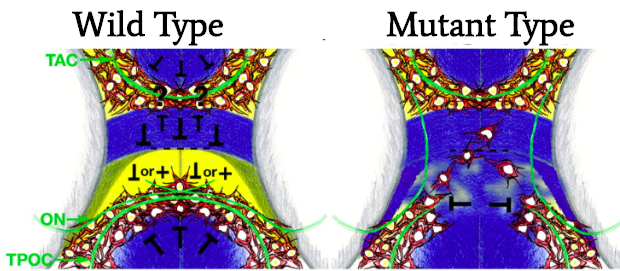
\includegraphics[width=0.9\linewidth]{visualization_paper/wt_yt} \caption{Wild-type and mutant-type commissure}\label{fig:Figure1}
\end{figure}

During the classification process, Dr.~Barresi's lab could only perform
categorization based on empirical knowledge. As a result, Morgan
Schwartz, a former lab member, wrote a Python program called \(\Delta\)
SCOPE to:\\
1. Align crooked 3D biological images so they could compare between
samples\\
2. Generate descriptive graphs with sample statistics\\
3. Classify samples into either wild type or mutant type based on the
statistics{[}1{]} {[}2{]}.

Our goal is to implement the Python program into R while maintaining and
improving as many features as possible. We modified existing functions
in \texttt{Cranium} package {[}3{]}, built new functions, and optimized
parameters so that evaluating sample alignments is no longer vulnerable
to subjective biases. Additionally, alignments will be able to run
automatically without labor-intensive manual correction that would
introduce more researcher biases.

\hypertarget{data}{%
\section{Data}\label{data}}

We received our data from Dr.~Jake Schnabl. The data files are brain
images of 43 wild-type samples and 35 mutant samples in HDF5 (.h5)
format. The data points stored within those files are marked using by
fluorescence microscopy, indicating neuronal signals. The data is
processed by an open-source software, Ilastik, before being read into R.
We are working with the data after being processed in Ilastik.

Raw image data was processed in \texttt{Illastik}. Each sample is
composed of data points, which are voxels of the image. Voxels stand for
volumetric pixels, which can be understood as the three-dimensional
equivalent of pixels. Each voxel has a frequency, representing the
probability of being a real signal.

\hypertarget{programming-languages}{%
\section{Programming Languages}\label{programming-languages}}

In this study, we used R in order to run algorithms, manipulate data,
and generate visualizations. For accessibility and reproducibility of
this research, we have stored our work on Github. {[}4{]}

\hypertarget{package-cranium}{%
\subsection{\texorpdfstring{Package
\texttt{Cranium}}{Package Cranium}}\label{package-cranium}}

The package \texttt{Cranium} contains several major functionalities
listed below:

\hypertarget{functionalities}{%
\section{Functionalities}\label{functionalities}}

\hypertarget{api}{%
\subsection{1.API}\label{api}}

The sample datasets for wild- and mutant-type are saved as \texttt{*.h5}
files. Originally, the lab had to share the data through a hard drive,
thus having a need for readily accessible data. In order to share the
data efficiently amongst users, the data is hosted on Amazon S3 with a
read only link to each sample. In the \texttt{Cranium} package,
functions were created that allows users to download an individual
sample or a bundle of samples. Each function downloads all existing
files onto the user's machine in a designated folder the user decides in
addition to outputting the list of samples of type brain class.

\hypertarget{tidy-data-and-threshold}{%
\subsection{2. Tidy Data and Threshold}\label{tidy-data-and-threshold}}

After reading the data, we organize the dataset using a tidy framework
for data manipulation, which has a specific structure: each row is an
observation and each column is a variable; in our case, \texttt{x,y,z}
coordinates {[}5{]}. After transforming the image data, each observation
in our data is a voxel, and each voxel contains information about how
strong that voxel is, which is referred to as frequency. Frequency
represents the probability of each voxel being a real signal. We want to
include as many ``real'' signals as possible while getting rid of voxels
that are very likely to be ``background noise.'' Therefore, we want to
set a threshold so that all the voxels that have frequencies below the
threshold are considered as noise and excluded from our analysis.

Wild-type samples and mutant-type samples originally contain different
number of voxels. Because of the deformed nature of mutant-type
commissures, mutant samples, on average, contain half or fewer voxels
than that of wild type. Also, compared to wild-type samples, mutant-type
samples' voxels generally have lower frequencies. Setting a high
threshold would not result in too small a sample size (i.e., signals)
for the wild type because the wild-type commissures are mostly formed
successfully and have relatively strong signals. However, a high
threshold would result in mutant-type sample having a very restricted
sample size because the wild-type commissures are mostly formed
successfully and have relatively strong signals.

For the purpose of research of Baressi's Lab, we want to compare wild-
and mutant-type sample, thus we have to set the same threshold for both
types of samples. A threshold of 0.9 was subjectively chosen previously
by observing the output of wild- and mutant-type samples, which raised
our concern of the validity of this threshold. Therefore, we decided to
1. test for the validity of this 0.9 threshold by examining model fit;
2. find a threshold that will optimize the model fit. We fit a quadratic
model on the x-y plane that captures the shape of the commissure, and we
use the adjusted \(R^2\) to evaluate the model fit. There are some
problems we encounter during the optimization process: having small
number of signals for mutant-type samples increases the chance of our
model overfitting the data; meanwhile, setting a low threshold for
mutant-type samples increases the the chance of noise to creep into the
dataset. Therefore, our goal is find the optimized threshold that fit
the data well by capturing the real signals, while ensuring that we have
enough mutant-type signals.

To find the optimal threshold, we test different thresholds and examine
their model fit according the following procedures:\\
1. Starting with one threshold, we fit one model to every single sample
and repeat fitting the model for all wild- and mutant-type samples. We
then evaluate the model fit at this specific threshold by respectively
taking the average \(R^2\) of the wild-type and of the mutant-type
samples.\\
2. Next, we repeat step 1. for other thresholds: \{0.4, 0.42, 0.44,
0.46, 0.48, 0.5, 0.52, 0.54, 0.56, 0.58, 0.6, 0.62, 0.64, 0.66, 0.7,
0.75, 0.8, 0.81, 0.82, 0.83, 0.84, 0.85, 0.86, 0.87, 0.88, 0.89, 0.90,
0.91, 0.92\}.\\
3. For each threshold, we generate a table of the threshold which we
listed at step 2. with its corresponding average adjusted \(R^2\) for
wild-type samples and average adjusted \(R^2\) for mutant-type samples.

In order to find the threshold that optimizes the average adjusted
\(R^2\) for both wild- and mutant-type samples, we generate a
scatterplot, as shown in Figure 2, for each threshold value, which is
represented by a distinct color. The use of lighter color indicates a
higher threshold. The size of each point represents the amount of
signals from the mutant-type sample that were captured by the model.
With x-axis representing the average mutant-type adjusted \(R^2\) and
y-axis representing the average wild-type adjusted \(R^2\), we are able
to find the optimal threshold.

\begin{figure}[H]
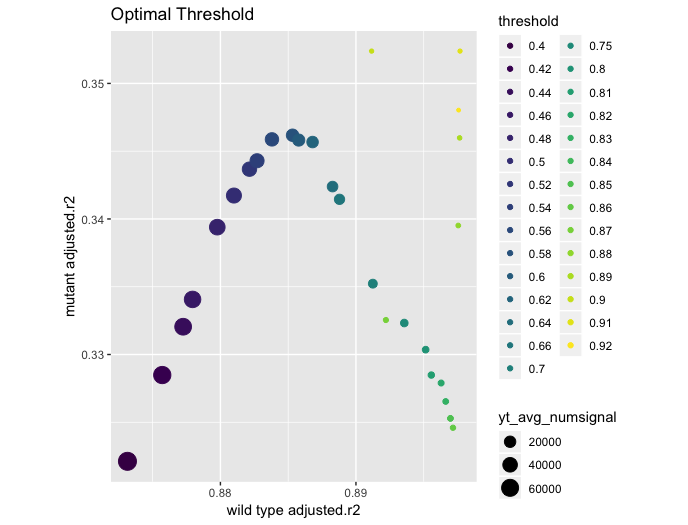
\includegraphics[width=0.9\linewidth]{visualization_paper/optimal_threshold2} \caption{Optimization of threshold for wild- and mutant-type samples}\label{fig:Figure2}
\end{figure}

We evaluate the performance of each threshold by comparing it to the
perfect model fit. A perfect model-fit for both wild- and mutant-type
samples should achieve an adjusted \(R^2 = 1\). In a two dimensional
space, we can find the Euclidean distance between the model fit of our
threshold and the perfect model fit. A smaller euclidean distance
indicates that we are closer to the perfect model fit.

\hypertarget{principal-component-analysis-pca-reorientation}{%
\subsection{3. Principal Component Analysis (PCA)
Reorientation}\label{principal-component-analysis-pca-reorientation}}

During the process of data collection, researchers took pictures of the
zebrafish brain under microscopes. We acknowledge that each of the
brains were in different positions and were placed in different angles.
Therefore, the pictures varied slightly in positioning. In order for us
to do further analyses and compare between samples, we need to re-orient
them using Principal Component Analysis (PCA) and identify a consistent
set of axes across all samples. In a three-dimensional space, PCA
assigns the axis with the most amount of variation as PC1 (first
principal component), then the axis with the second-most variation as
PC2, and lastly the axis with least amount of variation as PC3.
Afterwards, PCA picks the basis based on PC1, PC2, and PC2, which then
changes the positioning of the structure. As shown in Figure 3, we
graphically output three 2D planes in three perspectives: xy; yz; xz
planes. For the commissure, we would get three views: lateral;
dorsal/ventral; anterior/posterior. We set x axis as the lateral, y axis
as the anterior/posterior, and z as the dorsal/ventral.

\begin{figure}[H]
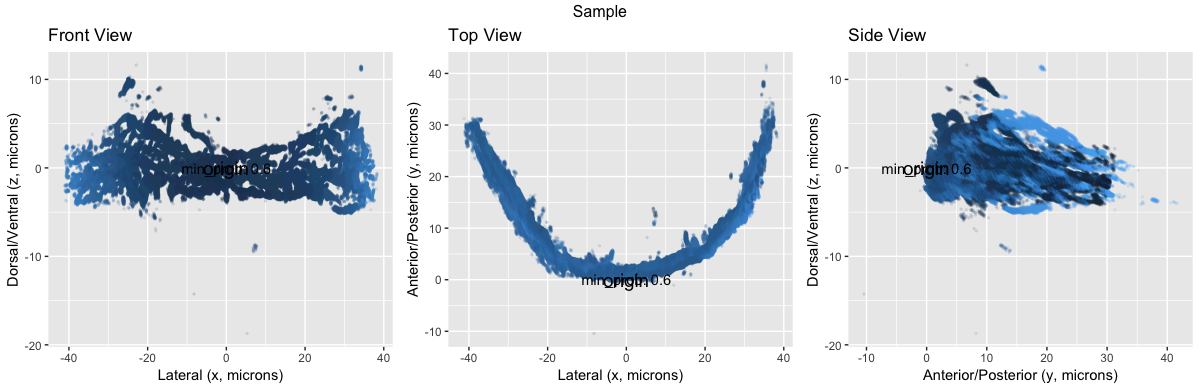
\includegraphics[width=1\linewidth]{visualization_paper/wt_04} \caption{2D plot of a wild-type sample}\label{fig:Figure3}
\end{figure}

\hypertarget{qmodel}{%
\subsection{4. Qmodel}\label{qmodel}}

We built the Qmodel function to fit a quadratic model to the data in
order to capture the shape of the commissure as well as evaluating model
fit. As shown in the Figure 4, the quadratic model fits on the xy-plane:
\(y=x^2+x\), indicated by red color. Our goal is to achieve a better
model fit. Qmodel outputs model statistics including: \(R^2\), adjusted
\(R^2\), sigmal (RSE), statistic, p.value, df, logLik, AIC, BIC,
deviance, df.residual, num.signal, quad.coeff, RMSE.

\begin{figure}[H]
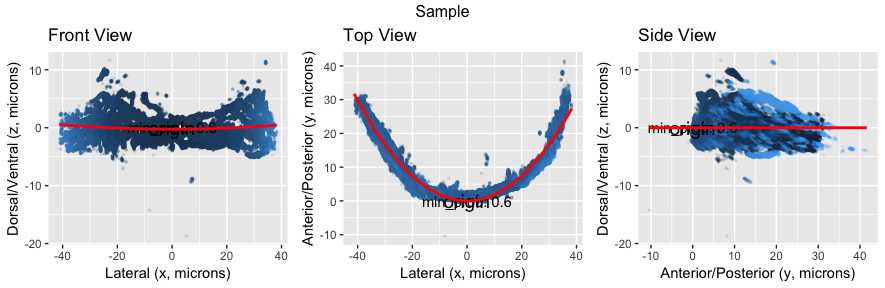
\includegraphics[width=1\linewidth]{visualization_paper/wt_04_model} \caption{Model fit on a wild-type sample}\label{fig:Figure4}
\end{figure}

\hypertarget{r2}{%
\subsubsection{\texorpdfstring{\(R^2\) :}{R\^{}2 :}}\label{r2}}

\(R^2\) is also called the coefficient of determination or the
coefficient of multiple determination for multiple regression. \(R^2\)
ranges from 0 to 1. It is calculated from the variance explained by the
model divided by total variance. Higher \(R^2\) values represent smaller
differences between the observed data and the fitted values, indicating
a better fit of the model. Note that \(R^2\) is a relative scale of
model fit.

\hypertarget{adjusted-r2}{%
\subsubsection{\texorpdfstring{Adjusted \(R^2\)
:}{Adjusted R\^{}2 :}}\label{adjusted-r2}}

Adjusted \(R^2\) is a modification of \(R^2\) and adjusts for the number
of predictors in the model.

\hypertarget{rmse-root-mean-squared-error}{%
\subsubsection{RMSE (Root Mean Squared
Error)}\label{rmse-root-mean-squared-error}}

gives the difference between observed data and model's predicted values.
Lower RMSE values represent smaller difference between observed data and
model's predicted values.

\hypertarget{num.signal}{%
\subsubsection{num.signal}\label{num.signal}}

It gives the number of signals being captured for the sample after
filter out the signals that are less than the threshold.

\hypertarget{quad.coeff}{%
\subsubsection{Quad.coeff}\label{quad.coeff}}

It is the coefficient of the \(x^2\) term in our model.

\hypertarget{pca-reorientation-correction}{%
\section{PCA Reorientation
Correction}\label{pca-reorientation-correction}}

Errors occur after the PCA reorientation, previously four errors were
identified in \(\Delta\)SCOPE. In our study, we identify two types of
error and make corresponding corrections, which is introduced in the
following section.

\hypertarget{systematic-correction-procedure}{%
\subsection{Systematic Correction
Procedure}\label{systematic-correction-procedure}}

Existing problem: previous research identified four types of errors.
However, users had to examine samples one at a time, subjectively make
decision on whether that sample has an error and then correct the error
with subjective judgment. We introduce a systematic correction procedure
as shown in Figure 5, striving to minimize user input in order to reduce
subjective biases, by making all the error identification and correction
automatic.

\begin{figure}[H]
\includegraphics[width=0.9\linewidth]{visualization_paper/Cranium_procedure} \caption{Systematic correction procedure}\label{fig:Figure5}
\end{figure}

\hypertarget{check-for-error-a-is_errora}{%
\subsubsection{\texorpdfstring{Check for error A--
\texttt{is\_errorA}}{Check for error A-- is\_errorA}}\label{check-for-error-a-is_errora}}

As shown in Figure 6, error A is identified as flipped y-axis, shown as
the solid curve in the xy-plane. A correct model fit a positive
quadratic model in the xy-plane, shown as the dotted curve. We fit a
quadratic model on the xy-plane: \(y=x^2 + x\). The positive quadratic
coefficient indicates a positive concavity; a negative quadratic
coefficient indicates a negative concavity. Having a negative quadratic
coefficient is resulted from an PCA reorientation error, which we
identify as error A. If error A occurs, the function will show ``Y Axis
is flipped'' and return ``TRUE''. If error A does not exist, then the
function will show ``Correct alignment'' and return ``FALSE''.

\begin{figure}[H]
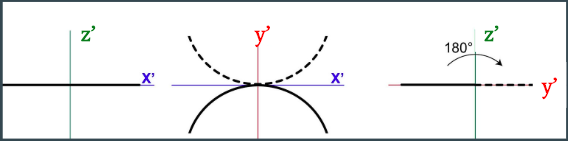
\includegraphics[width=0.9\linewidth]{visualization_paper/error_correctionA} \caption{Error A in 3-D}\label{fig:Figure6}
\end{figure}

\hypertarget{error-a-correction-correct_errora}{%
\subsubsection{\texorpdfstring{Error A correction --
\texttt{correct\_errorA}}{Error A correction -- correct\_errorA}}\label{error-a-correction-correct_errora}}

If a sample data returned TRUE for error A, the function then changes
the sign of the y-value of all the data points, as a result flipping the
y-axis. As shown in the following code, originally y = y -
vertex{[}2{]}. We flipped the y-axis by reversing its value: y =
vertex{[}2{]} - y.

\begin{Shaded}
\begin{Highlighting}[]
\ControlFlowTok{if}\NormalTok{ (correctionA }\OperatorTok{==}\StringTok{ }\OtherTok{TRUE}\NormalTok{)\{}
\NormalTok{    data <-}\StringTok{ }\NormalTok{data }\OperatorTok
\StringTok{      }\KeywordTok{mutate}\NormalTok{(}\DataTypeTok{x =}\NormalTok{ x }\OperatorTok{-}\StringTok{ }\NormalTok{vertex[}\DecValTok{1}\NormalTok{], }\DataTypeTok{y =}\NormalTok{  vertex[}\DecValTok{2}\NormalTok{] }\OperatorTok{-}\StringTok{ }\NormalTok{y , }\DataTypeTok{z =}\NormalTok{ z }\OperatorTok{-}\StringTok{ }\NormalTok{z_mean}\OperatorTok{$}\NormalTok{z_mean)}
\NormalTok{  \} }\ControlFlowTok{else}\NormalTok{ \{}
\NormalTok{    data <-}\StringTok{ }\NormalTok{data}\OperatorTok
\StringTok{      }\KeywordTok{mutate}\NormalTok{(}\DataTypeTok{x =}\NormalTok{ x }\OperatorTok{-}\StringTok{ }\NormalTok{vertex[}\DecValTok{1}\NormalTok{], }\DataTypeTok{y =}\NormalTok{ y }\OperatorTok{-}\StringTok{ }\NormalTok{vertex[}\DecValTok{2}\NormalTok{], }\DataTypeTok{z =}\NormalTok{ z }\OperatorTok{-}\StringTok{ }\NormalTok{z_mean}\OperatorTok{$}\NormalTok{z_mean)}
\NormalTok{  \}}
\end{Highlighting}
\end{Shaded}

\hypertarget{check-for-error-b-is_errorb}{%
\subsubsection{\texorpdfstring{Check for error B --
\texttt{is\_errorB}}{Check for error B -- is\_errorB}}\label{check-for-error-b-is_errorb}}

Error B is identified as having curvature in the xy-plane as shown in
Figure 7. A correct PCA orientation will output a horizontal, flat
linear line in xz-plane, meaning that the quadratic coefficient for the
quadratic model in the xz-plane is zero. However, it is not practical to
expect the quadratic coefficient to be perfectly zero with no variance.
Therefore, we construct a normal range for the quadratic coefficient. We
achieve good quadratic model fit for wild-type samples, having adjusted
\(R^2 > 0.85\). Also, we do not observe an obvious curvature of the data
points in the xz-plane. Thus, we use wild-type samples as our reference
group to construct the normal range for the quadratic coefficient.

\begin{figure}[H]
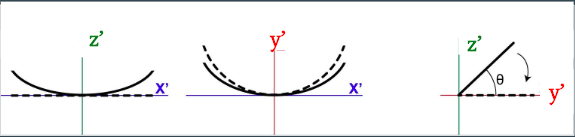
\includegraphics[width=0.9\linewidth]{visualization_paper/error_correctionB} \caption{Error B in 3-D}\label{fig:Figure7}
\end{figure}

To do this, we first identify the standard error of the quadratic
coefficient for all of our wild-type samples. Then, we construct a
range: (mean - standard error, mean + standard error) as the range of
``acceptable'' curvature for wild-type samples. Then, we check whether
the quadratic coefficient of each mutant sample is within that range. If
it is, we would consider the curvature of that mutant sample acceptable,
meaning that there is not an error B for that sample. If the quadratic
coefficient of a mutant sample is not within the acceptable range, we
would then consider that there exists an error B in the sample.

We introduce three different ranges to be considered as a normal
range:\\
1. Interquartile Range (IQR), calculated as the difference of quartile
three and quartile one. Quantile 1 as the lower bound and quantile 3 as
the upper bound.\\
2. Outlier range, calculated from the IQR. \texttt{mean\ -\ 1.5*IQR} as
the lower bound and \texttt{mean\ +\ 1.5*IQR} as the upper bound. Any
data that's outside this range is considered as outlier.\\
3. 95\% Confidence interval.

As shown in Figure 8. The range between the two blue lines indicates the
outlier range, followed by red lines as IQR range, and then green lines
as 95\% confidence interval. We set the outlier range as our default
range. Users are able to decide which type of range they want to use.
With a wider range, more wild-type samples will be identified in the
normal range and more mutant-type samples will be identified in the
normal range.

\begin{figure}[H]
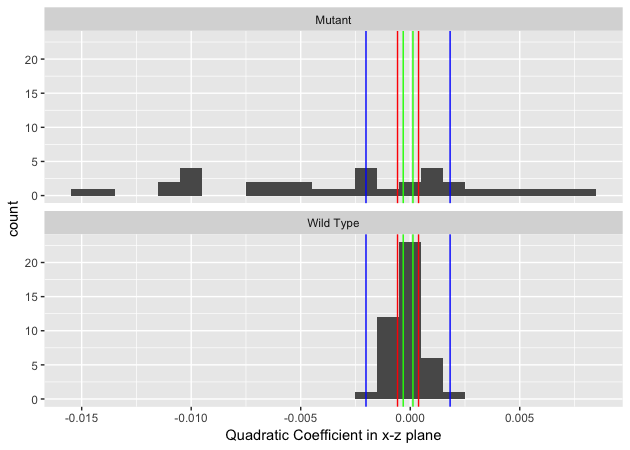
\includegraphics[width=0.9\linewidth]{visualization_paper/range_for_is_errorB} \caption{Normal range of the quadratic coefficient}\label{fig:Figure8}
\end{figure}

\hypertarget{error-b-correction---correct_errorb}{%
\subsubsection{\texorpdfstring{Error B correction -
\texttt{correct\_errorB}}{Error B correction - correct\_errorB}}\label{error-b-correction---correct_errorb}}

Figure 9 shows our rotation method.

\begin{figure}[H]
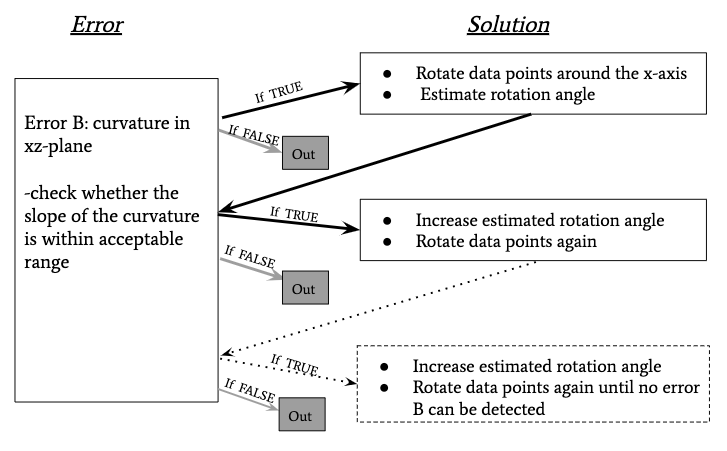
\includegraphics[width=0.9\linewidth]{visualization_paper/diagram_2errors} \caption{Procedures for checking and correcting error B}\label{fig:Figure9}
\end{figure}

After identifying the curvature in the xz-plane, we correct the error by
rotating data points a certain angle around the x-axis.

\hypertarget{step-1.-first-we-use-alpha-to-estimate-rotation-angle-theta}{%
\paragraph{\texorpdfstring{Step 1. First, we use \(\alpha\) to estimate
rotation angle
\(\theta\)}{Step 1. First, we use \textbackslash{}alpha to estimate rotation angle \textbackslash{}theta}}\label{step-1.-first-we-use-alpha-to-estimate-rotation-angle-theta}}

As shown in Figure 10, we fit a quadratic model on the xz-plane
\(z=x^2+x\). \(\theta\) is our rotation angle. All the data points are
rotated \(\theta\) degree around the x-axis in order to correct error B
in order to flatten the curvature in the xz-plane. Since the dotted line
\(l1\) is parallel to \(l3\), angle \(\beta\) = \(\alpha\) according to
a parallel-line-theorem, which states that ``if lines are parallel and
cut by a transversal line, then the corresponding angles are equal''.
Thus, we are able to use \(\alpha\) to estimate our rotation angle
\(\theta\).

\begin{figure}[H]
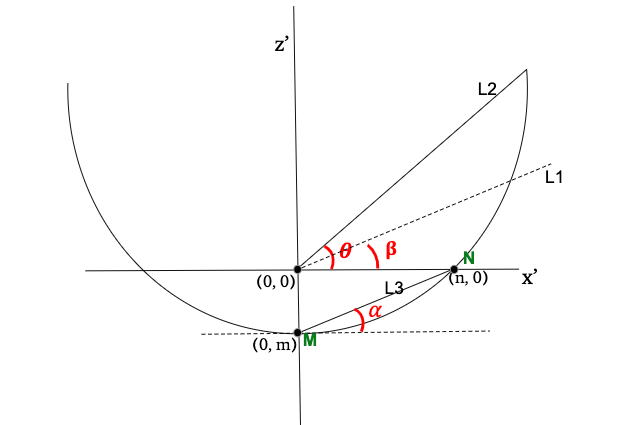
\includegraphics[width=0.9\linewidth]{visualization_paper/rotation_angle} \caption{Rotation angle estimation}\label{fig:Figure10}
\end{figure}

\hypertarget{step-2.-find-alpha}{%
\paragraph{\texorpdfstring{Step 2. Find
\(\alpha\)}{Step 2. Find \textbackslash{}alpha}}\label{step-2.-find-alpha}}

Let the quadratic equation to be \(y=ax^2 + bx +c\). Let \(a\) to be the
quadratic coefficient, let \(b\) to be the slope, let \(c\) to be the
intercept. We can find the y intercept by setting \(x=0\). Similarly, we
calculate the x intercept using this formula:
\[\frac{-b-sqrt(b^2-4ac)}{2a}\] We only consider the positive
x-intercept here since the x-intercepts are symmetric about y-axis,
which serve their purposes the same.

Let M be the y-intercept with coordinate \((0, m)\). Let N be the
x-intercept with coordinate \((n, 0)\). We can use formula
\[\frac{y2-y1}{x2-x1}\] to find the slope of \(l3\), which connects
points M and N. After simplification, we get the slope of L3 to be
\(\frac{m}{n}\). We use the formula angle =\(tan^{-1} \times\) slope of
a line to find the angle \(\alpha\).

\hypertarget{step-3.-use-the-estimated-angle-alpha-to-perform-rotation}{%
\paragraph{\texorpdfstring{Step 3. Use the estimated angle \(\alpha\) to
perform
rotation}{Step 3. Use the estimated angle \textbackslash{}alpha to perform rotation}}\label{step-3.-use-the-estimated-angle-alpha-to-perform-rotation}}

We rotate our data points around the x-axis by performing matrix
multiplication: multiplying our current data with the rotation matrix
\(R_z(\theta)\) shown in Figure 11. \(\theta\) in the \(R_z\) is the
rotation angle. We plug in our estimated rotation angle \(\alpha\) into
the rotation matrix \(R_z(\theta)\).

\begin{figure}[H]
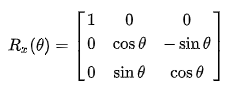
\includegraphics[width=0.3\linewidth]{visualization_paper/rotation_matrix} \caption{Rotation matrix}\label{fig:Figure11}
\end{figure}

We convert our dataframe to a matrix with dimensions \(n \times 3\),
where n is the number of data points in a dataframe. We then multiply
our \(n \times 3\) data matrix by our rotation matrix. The output is a
matrix with rotated data points in dimension \(n \times 3\).

\hypertarget{step-4.-evaluation-and-reorientation}{%
\paragraph{Step 4. Evaluation and
reorientation}\label{step-4.-evaluation-and-reorientation}}

We check whether the reoriented data has error B, if there is an error,
we will re-apply the rotation by doubling the rotation angle until we
are cleared for error B. Every time we re-apply the rotation, we
increase the rotation angle: for the \(i^{th}\) time of re-orientation,
we would multiply \(i^{th}\) to our original rotation angle \(\alpha\).

\hypertarget{results}{%
\section{Results}\label{results}}

\hypertarget{threshold-optimization-evaluation}{%
\subsection{1. Threshold Optimization
Evaluation}\label{threshold-optimization-evaluation}}

\hypertarget{a.-number-of-signals}{%
\subsubsection{a. Number of signals}\label{a.-number-of-signals}}

Different thresholds will leave us with different number of signals per
sample. Figure 12 shows us the boxplot of the average number of signals
for wild- and mutant-type samples at each threshold. For each threshold,
wild-type samples have a lot more number of signals than mutant-type
samples. Note that at threshold 0.9, the average number of signals for
mutant-type samples almost equal to zero. At threshold of 0.92, we find
that some mutant-type samples do not have any signals left. In the
following section, we will compare the model fit for wild-type samples
and mutant samples at each threshold.

\begin{figure}[H]
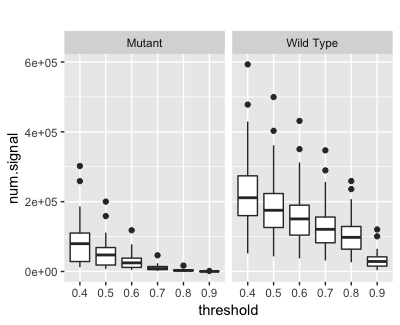
\includegraphics[width=0.6\linewidth]{visualization_paper/thresh_numsig_boxplot} \end{figure}

\hypertarget{b.-optimal-threshold-for-wild--and-mutant-type-samples}{%
\subsubsection{b. Optimal threshold for wild- and mutant-type
samples}\label{b.-optimal-threshold-for-wild--and-mutant-type-samples}}

We use Qmodel, a quadratic model fitted on the xy-plane, to evaluate
model performance at each threshold. First, we fit the \texttt{Qmodel}
on all samples. For each threshold, we take an average of the adjusted
\(R^2\) for all wild-type samples, and an average of the adjusted
\(R^2\) for all mutant-type samples.

Figure 13 shows the model adjusted \(R^2\) at different thresholds for
wild- and mutant-type samples. The model fits pretty well on wild-type
samples in general: majority of the samples achieve adjusted
\(R^2 > 0.75\). However, for mutant samples, not only does the model not
perform ideally, but the variance of the adjusted \(R^2\) for the
samples at each threshold is high. Based on the averaged adjusted
\(R^2\), we observe that the thresholds between 0.87 to 0.9 yield the
best model fit for wild-type samples, whereas we are not able to
determine a threshold that yields the best model fit for mutant samples.

\begin{figure}[H]
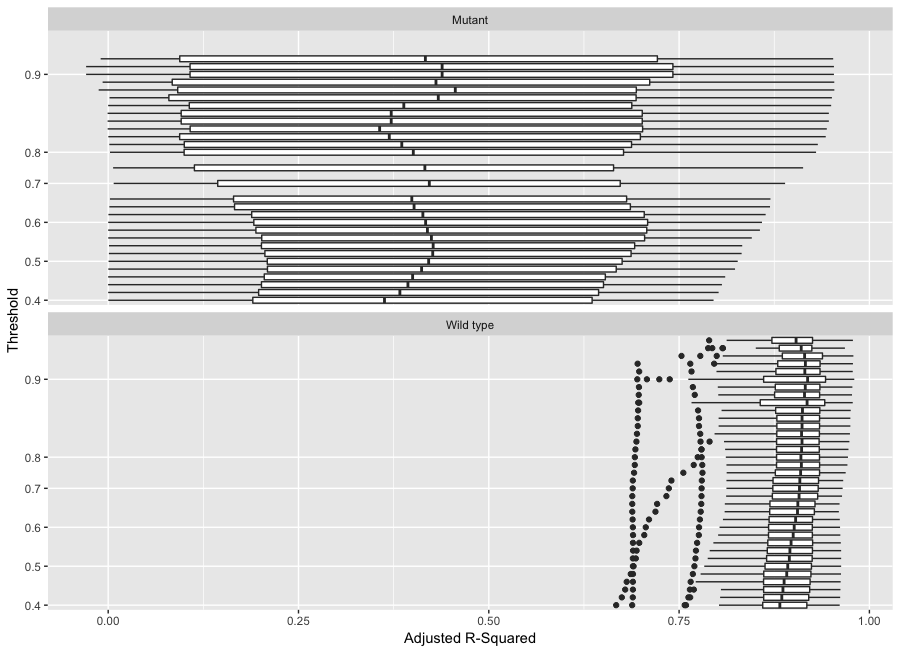
\includegraphics[width=0.9\linewidth]{visualization_paper/threshold_boxplot} \caption{Adjusted R2 comparison for different threshold for wild-and mutant-type samples}\label{fig:Figure13}
\end{figure}

\hypertarget{c.-find-optimal-threshold-for-both-wild--and-mutant-type-samples}{%
\subsubsection{c. Find optimal threshold for both wild- and mutant-type
samples}\label{c.-find-optimal-threshold-for-both-wild--and-mutant-type-samples}}

In order to compare wild- and mutant-type samples, the threshold needs
to be the same for both types. As mentioned in the Functionalities
section earlier, Euclidean distance is used to compare the performance
of the model on our sample for each threshold with the perfect model
fit. We calculate this Euclidean distance to determine the optimal
threshold for both types of samples. The Figure 2 shows that the
thresholds between 0.90 and 0.92 achieve the optimal model fit, having
the smallest Euclidean distance. However, as mentioned in section ``a.
Number of signals'', the average number of signals of mutant-type
samples is very low once threshold reaches 0.9. At threshold=0.9, the
average number of signals of mutant-type samples drops to 303 (\(SD\) =
299), which poses a threat of the model overfitting the data.
Overfitting underestimate the true error of the data, which occurs in
our case when the sample size is small. In order to avoid overfitting
our data, we want to ensure that for each sample there are enough number
of signals. As shown in Figure 2, threshold of 0.6 is located at the
peak of the curve, which is the threshold that gives the smallest
Euclidean distance after 0.9 to 0.92 thresholds. Thus, we propose a new
optimal threshold of 0.6.

\hypertarget{pca-reorientation-model-fit-evaluation}{%
\subsection{2. PCA Reorientation Model Fit
Evaluation}\label{pca-reorientation-model-fit-evaluation}}

We compare the adjusted \(R^2\) of the model before and after PCA
reorientation, and we find that PCA transformation significantly
improved the model fit.

For Figures 14 and 15 each point represents a wild-type sample or a
mutant-type sample. The x-axis gives the adjusted \(R^2\) before PCA
reorientation and the y-axis gives the adjusted \(R^2\) after PCA
reorientation. The red line \(y=x\) is plotted in both figures, which
informs whether the PCA improves the quadratic model fit: the samples
below the red line perform worse after the PCA reorientation and the
samples above the red line perform better after the PCA reorientation.

\begin{figure}[H]
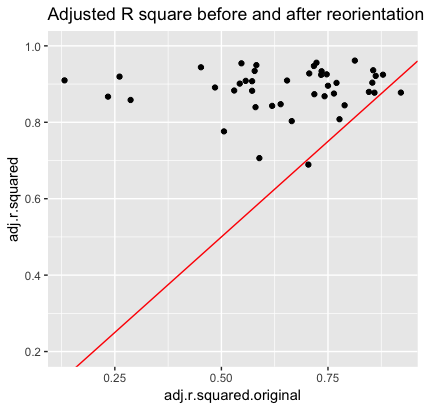
\includegraphics[width=0.6\linewidth]{visualization_paper/adj_r2_before_after_wt} \caption{PCA }\label{fig:Figure14}
\end{figure}

\begin{figure}[H]
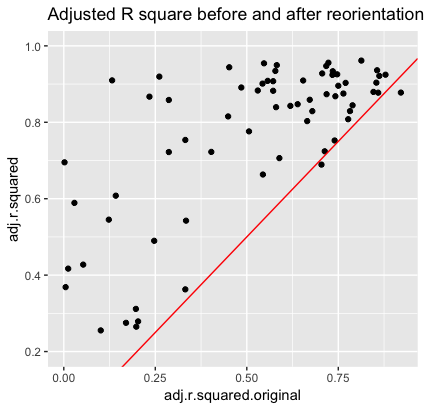
\includegraphics[width=0.6\linewidth]{visualization_paper/adj_r2_before_after_yt} \end{figure}

In order to compare the difference in the model fit before and after PCA
reorientation, we perform paired sample t-tests on wild- and mutant-type
samples for threshold 0.6.

\begin{Shaded}
\begin{Highlighting}[]
\KeywordTok{t.test}\NormalTok{(data}\OperatorTok{$}\NormalTok{adj.r.squared.original, data}\OperatorTok{$}\NormalTok{adj.r.squared, }\DataTypeTok{paired =} \OtherTok{TRUE}\NormalTok{, }
       \DataTypeTok{alternative =} \StringTok{"two.sided"}\NormalTok{)}
\end{Highlighting}
\end{Shaded}

For wild-type samples, the adjusted \(R^2\) after PCA reorientation is
significantly higher than the average adjusted \(R^2\) before PCA
reorientation with a p-value =\(5.765^{-10}\). For mutant-type samples,
it was found that the adjusted \(R^2\) after PCA reorientation is
significantly higher than the average adjusted \(R^2\) before PCA
reorientation with a p-value = \(1.863^{-4}\). The result demonstrates
the importance of PCA reorientation.

PCA reorientation performs better on the wild-type samples. As shown in
the Figure 14 and Figure 15, for both wild- and mutant- type samples,
those with high original adjusted \(R^2\)s have much higher adjusted
\(R^2\)s after the PCA reorientation. Wild-type samples with low
original adjusted \(R^2\)s have much higher adjusted \(R^2\)s after the
PCA reorientation. However, many mutant-type samples with low original
adjusted \(R^2\)s only achieve slight improvements on their adjusted
\(R^2\)s.

\hypertarget{conclusion}{%
\section{Conclusion}\label{conclusion}}

\hypertarget{conclusion-1}{%
\subsection{Conclusion}\label{conclusion-1}}

The three major improvements we make in the \texttt{Cranium}
functionalities include:\\
1. Data accessibility\\
2. Reduce user bias: minimize user input, reduce user bias\\
3. Easy for researchers to explore the data

In recent years, more researchers aim to produce reproducible and
open-source results. By storing the data using an API key, we solve the
problem of physically transferring the data using hard drives and
therefore making it possible for more researchers to examine zebrafish
commissure structures using the same data. We implement a systematic
optimization process to reduce user input, therefore minimizing the
amount of subjectivity involved in the data reorientation process. Also,
\texttt{Cranium} is easier to manipulate and requires little background
in programming languages to use. As a result, it allows and encourages
life science researchers to analyze 3D data independently.

\hypertarget{future-research}{%
\subsection{Future research}\label{future-research}}

PCA alignment error detection and correction could be optimized in the
future. After the correction A, which addresses the flipped y-axis error
and correction B, which addresses the curvature in the xz-plane problem,
we would like to see whether the quadratic model fit on our wild- and
mutant-type samples would be improved from the model fit on the samples
before our corrections.

\hypertarget{references}{%
\section*{References}\label{references}}
\addcontentsline{toc}{section}{References}

\hypertarget{refs}{}
\leavevmode\hypertarget{ref-Schwartz18}{}%
1. M. Schwartz BB J. Schnab. A new computational method to quantify
3D383image data and to detail changes in morphological structure and
spatial384relationships during nervous system development. 2018;

\leavevmode\hypertarget{ref-Hu18}{}%
2. S. Hu DT W. Li. Classification of wild type and mutant zebrafish
brains viaComputational method. 2018;

\leavevmode\hypertarget{ref-cranium}{}%
3. Benjamin Baumer EN Ziwei Crystal Zang. Cranium: Quantifying radial
bridge structures. 2019.

\leavevmode\hypertarget{ref-rticles19}{}%
4. Allaire J, Xie Y, R Foundation, Wickham H, Journal of Statistical
Software, Vaidyanathan R, et al. Rticles: Article formats for r markdown
{[}Internet{]}. 2019. Available:
\url{https://CRAN.R-project.org/package=rticles}

\leavevmode\hypertarget{ref-tidy-data}{}%
5. Wickham H. Tidy data. The Journal of Statistical Software. 2014;59.
Available: \url{http://www.jstatsoft.org/v59/i10/}

\nolinenumbers


\end{document}

